\chapter{Algebra Boole'a}

\begin{definicja}
\textbf{\emph{Algebra Boole'a}}\index{algebra!Boole'a} to struktura algebraiczna (Def. \ref{def:struktura_algebraiczna}, str. \pageref{def:struktura_algebraiczna})

\[
\mathbb{B} = \left(\mathbf{B}, \cup, \cap, \overline{\phantom{0}}, 0, 1\right),
\]

\noindent w kt�rej

\begin{itemize}
\item $\cup$ i $\cap$ s� dzia�aniami dwuargumentowymi,
\item $\overline{\phantom{0}}$ jest dzia�aniem jednoargumentowym,
\item a $0$ i $1$ s� \emph{wyr�nionymi, r�nymi} elementami zbioru $\mathbf{B}$,
\end{itemize}

\medskip

\noindent spe�niaj�ca nast�puj�ce warunki:

\begin{enumerate}
\item dzia�anie $\cup$ jest \textbf{przemienne} (Def. \ref{def:dzialanie_przemienne}, str. \pageref{def:dzialanie_przemienne})
\item dzia�anie $\cup$ jest \textbf{��czne} (Def. \ref{def:dzialanie_laczne}, str. \pageref{def:dzialanie_laczne})
\item aksjomat Huntingtona\index{aksjomat!Huntingtona}: 

\[
\forall \: x, y \in B \qquad \Rightarrow \qquad \overline{\left( \overline{x} \cup \overline{y} \right)} \cup \overline{\left(\overline{x} \cup y \right)} \; = \; x
\]
\end{enumerate}
\end{definicja}

\medskip

\begin{definicja}
\textbf{\emph{Elementem jednostkowym}}\label{def:element_jednostkowy} nazywamy element $\mathbf{1}$ taki, �e:

\[
\forall \: x \in B \colon \qquad x \cup \overline{x} \; = \; \mathbf{1}
\]
\end{definicja}

\medskip

\begin{definicja}
\textbf{\emph{Elementem zerowym}}\label{def:element_zerowy} nazywamy element $\mathbf{0}$ taki, �e:

\[
\forall \: x \in B \colon \qquad \overline{x \cup \overline{x}} \; = \; \mathbf{0}
\]
\end{definicja}

\medskip

\begin{definicja}
\textbf{\emph{Dzia�anie $\cap$}}:
\[
\forall \; x,y \in B \colon \qquad x \cap y \; = \; \overline{\overline{x} \cup \overline{y}}
\]
\end{definicja}

\bigskip

%%%%%%%%%%%%%%%%%%%%%%%%%%%
\section{Tabela dzia�a�}

$\alpha$, $\beta$ - zdania (formy zdaniowe, kt�rym mo�na przypisa� warto��)

\medskip

\begin{tabular}{|c|c|c|c|c|c|c|}
\hline
$\alpha$ & $\beta$ & $\overline{\alpha}$ & $\alpha \vee \beta$ & $\alpha \wedge \beta$ & $\alpha \Rightarrow \beta$ & $\alpha \Leftrightarrow \beta$ \\
\hline
0 & 0 & 1 & 0 & 0 & 1 & 1 \\
0 & 1 & 1 & 1 & 0 & 1 & 0 \\
1 & 0 & 0 & 1 & 0 & 0 & 0 \\
1 & 1 & 0 & 1 & 1 & 1 & 1 \\
\hline
\end{tabular}

\bigskip
%%%%%%%%%%%%%%%%%%%%%%%%%%%%%%%%%%%%%%%%%%%%
\section{Twierdzenia dla Algebry Boole'a}

\begin{twierdzenie}[o unikalno�ci]
Jest \textbf{tylko jeden} element jednostkowy~$\mathbf{1}$ (Def. \ref{def:element_jednostkowy}, str. \pageref{def:element_jednostkowy}).

Jest \textbf{tylko jeden} element zerowy~$\mathbf{0}$ (Def. \ref{def:element_zerowy}, str. \pageref{def:element_zerowy}).
\end{twierdzenie}

\medskip

\begin{twierdzenie}[o dope�nianiu]
\[
x \cup \overline{x} \; = \; \mathbf{1}
\]
\[
x \cap \overline{x} \; = \; \mathbf{0}
\]
\end{twierdzenie}

\medskip

\begin{twierdzenie}[o podw�jnej negacji]
\[
\overline{\overline{x}} \; = \; x
\]
\end{twierdzenie}

\medskip

\begin{twierdzenie}[prawa De Morgana]
\[
\overline{x \cup y} \; = \; \overline{x} \cap \overline{y}
\]
\[
\overline{x \cap y} \; = \; \overline{x} \cup \overline{y}
\]
\end{twierdzenie}

\medskip

\begin{twierdzenie}
\[
x \cap x \; = \; x
\quad
x \cup x \; = \; x
\quad
x \cup \mathbf{0} \; = \; x
\quad
x \cup \mathbf{1} \; = \; \mathbf{1}
\quad
x \cap \mathbf{1} \; = \; x
\quad
x \cap \mathbf{0} \; = \; \mathbf{0}
\]
\end{twierdzenie}

\medskip

\begin{twierdzenie}[o rozdzielno�ci]
\[
x \cup \left(y \cap z \right) \; = \; \left(x \cup y \right) \cap \left(x \cup z \right)
\]
\[
x \cap \left(y \cup z\right) \; = \; \left(x \cap y\right) \cup \left(x \cap z\right)
\]
\end{twierdzenie}

\bigskip
%%%%%%%%%%%%%%%%%%%%%%%%%%%%%%%%%%%%%%%%%%%%%%%%%%%%%%%%
\section{Funktory w elektrotechnice. Bramki logiczne}

\smallskip
%%%%%%%%%%%%%%%%%%%%%%%%%%
\subsection{Bramka NOT}
\index{bramka!NOT}

\begin{tabular}{m{6cm}m{7cm}m{0.1cm}}
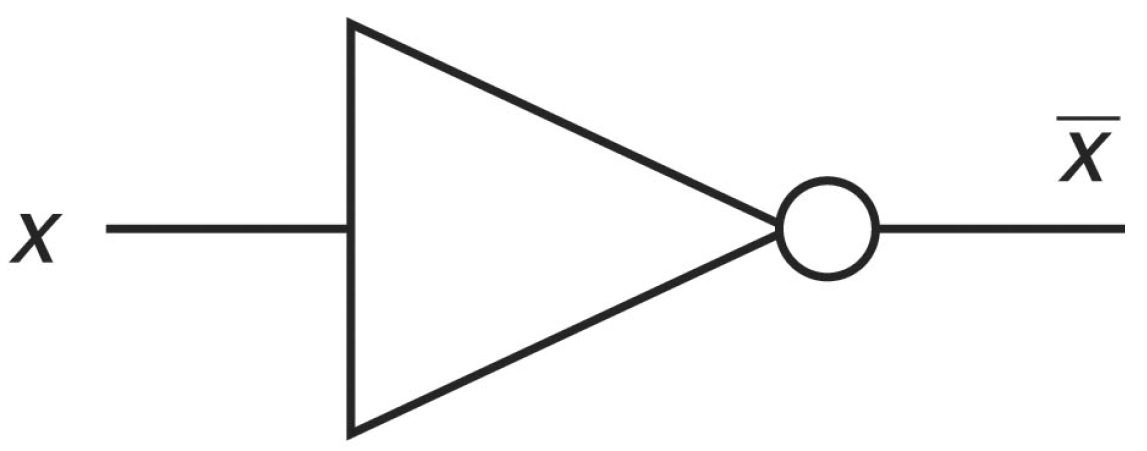
\includegraphics[width=4cm]{img/gates-not.png} &
\begin{tabular}{|m{1cm}|m{1cm}|m{0.1cm}}
\cline{1-2} $x$ & $\overline{x}$ &\\[1em]
\cline{1-2} 0 & 1 &\\[0.3em]
1 & 0 &\\[0.3em]
\cline{1-2}
\end{tabular}
& \\
\end{tabular}


\bigskip
%%%%%%%%%%%%%%%%%%%%%%%%%
\subsection{Bramka OR}
\index{bramka!OR}

\begin{tabular}{m{6cm}m{7cm}m{0.1cm}}
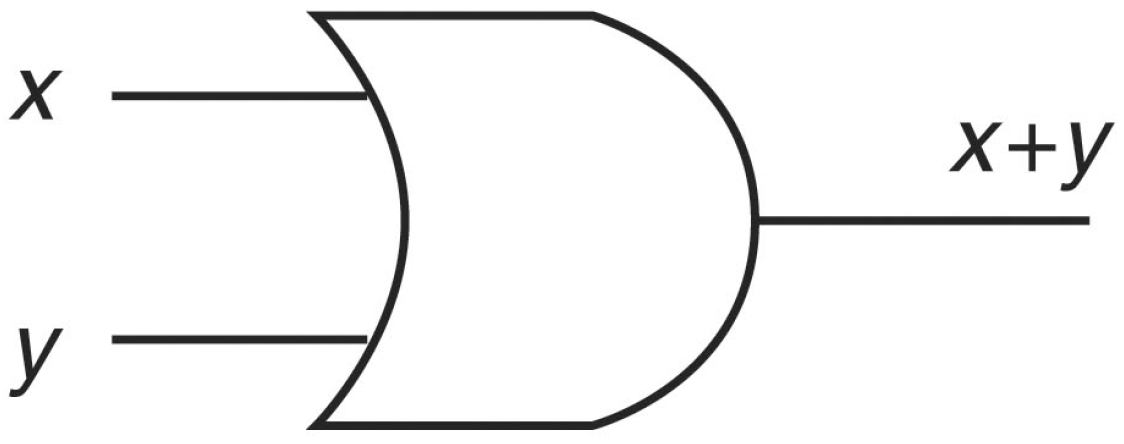
\includegraphics[width=4cm]{img/gates-or.png} &
\begin{tabular}{|m{1cm}|m{1cm}|m{1cm}|m{0.1cm}}
\cline{1-3} $x$ & $y$ & $x \vee y$ &\\[1em]
\cline{1-3} 0 & 0 & 0 &\\[0.3em]
0 & 1 & 1 &\\
1 & 0 & 1 &\\
1 & 1 & 1 &\\[0.3em]
\cline{1-3}
\end{tabular}
& \\
\end{tabular}

\bigskip
%%%%%%%%%%%%%%%%%%%%%%%%%%
\subsection{Bramka NOR}
\index{bramka!NOR}

\begin{tabular}{m{6cm}m{7cm}m{0.1cm}}
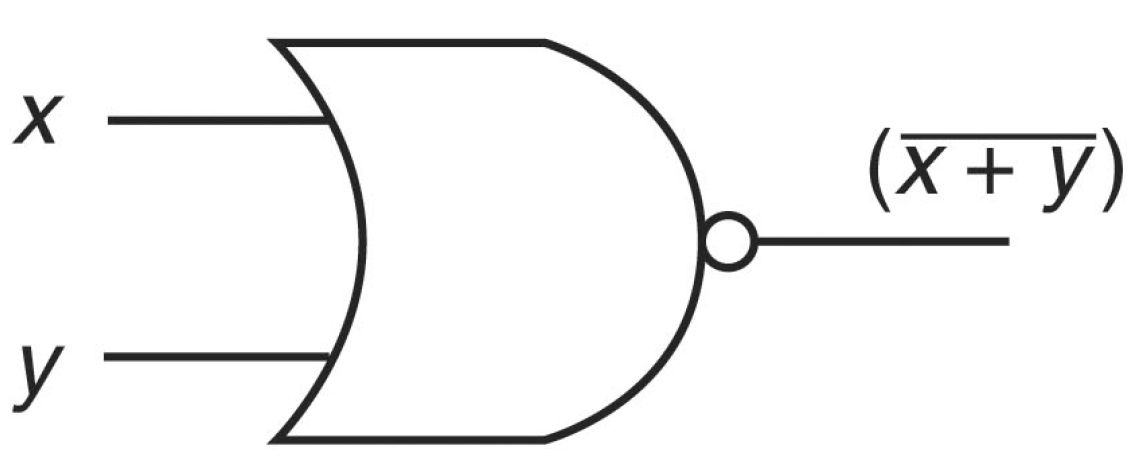
\includegraphics[width=4cm]{img/gates-nor.png} &
\begin{tabular}{|m{1cm}|m{1cm}|m{1cm}|m{0.1cm}}
\cline{1-3} $x$ & $y$ & $\overline{x \vee y}$ &\\[1em]
\cline{1-3} 0 & 0 & 1 &\\[0.3em]
0 & 1 & 0 &\\
1 & 0 & 0 &\\
1 & 1 & 0 &\\[0.3em]
\cline{1-3}
\end{tabular}
& \\
\end{tabular}


\bigskip
%%%%%%%%%%%%%%%%%%%%%%%%%%
\subsection{Bramka AND}
\index{bramka!AND}

\begin{tabular}{m{6cm}m{7cm}m{0.1cm}}
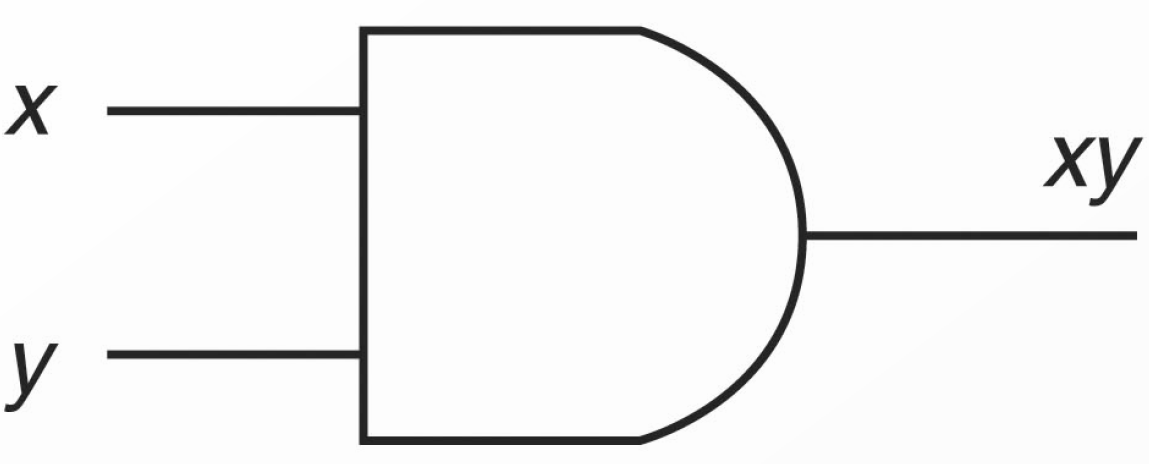
\includegraphics[width=4cm]{img/gates-and.png} &
\begin{tabular}{|m{1cm}|m{1cm}|m{1cm}|m{0.1cm}}
\cline{1-3} $x$ & $y$ & $x \wedge y$ &\\[1em]
\cline{1-3} 0 & 0 & 0 &\\[0.3em]
0 & 1 & 0 &\\
1 & 0 & 0 &\\
1 & 1 & 1 &\\[0.3em]
\cline{1-3}
\end{tabular}
& \\
\end{tabular}

\bigskip
%%%%%%%%%%%%%%%%%%%%%%%%%%%
\subsection{Bramka NAND}
\index{bramka!NAND}

\begin{tabular}{m{6cm}m{7cm}m{0.1cm}}
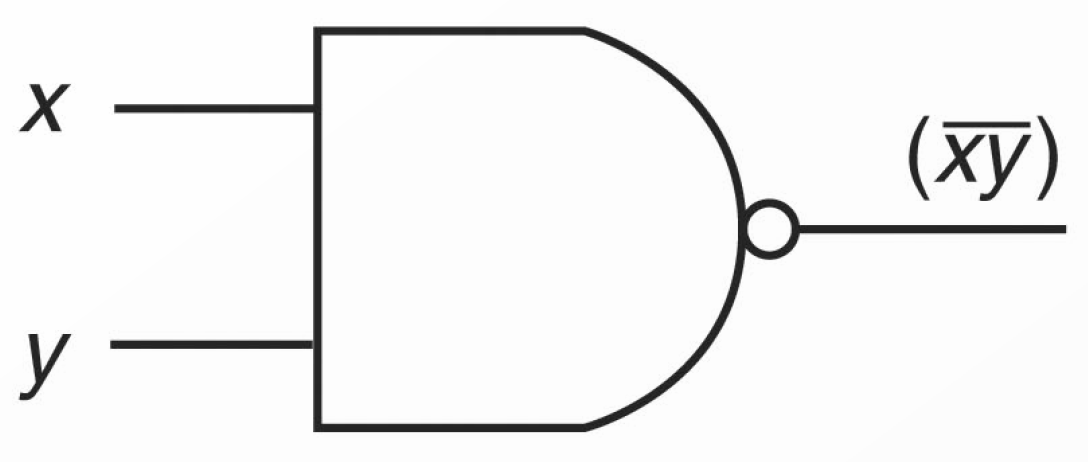
\includegraphics[width=4cm]{img/gates-nand.png} &
\begin{tabular}{|m{1cm}|m{1cm}|m{1cm}|m{0.1cm}}
\cline{1-3} $x$ & $y$ & $\overline{x \wedge y}$ &\\[1em]
\cline{1-3} 0 & 0 & 1 &\\[0.3em]
0 & 1 & 1 &\\
1 & 0 & 1 &\\
1 & 1 & 0 &\\[0.3em]
\cline{1-3}
\end{tabular}
& \\
\end{tabular}

\bigskip
%%%%%%%%%%%%%%%%%%%%%%%%%%
\subsection{Bramka XOR}
\index{bramka!XOR}

\begin{tabular}{m{6cm}m{7cm}m{0.1cm}}
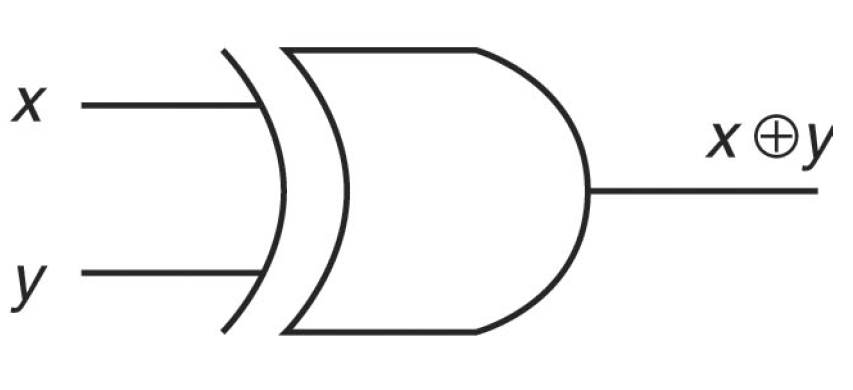
\includegraphics[width=4cm]{img/gates-xor.png} &
\begin{tabular}{|m{1cm}|m{1cm}|m{1cm}|m{0.1cm}}
\cline{1-3} $x$ & $y$ & $x \underline{\vee} y$ &\\[1em]
\cline{1-3} 0 & 0 & 0 &\\[0.3em]
0 & 1 & 1 &\\
1 & 0 & 1 &\\
1 & 1 & 0 &\\[0.3em]
\cline{1-3}
\end{tabular}
& \\
\end{tabular}

